\cleardoublepage
\chapter{Principio di equivalenza}
\label{cha:principio-equivalenza}

\section{Principio di equivalenza}
\label{sec:principio-equivalenza}

\subsection{Massa inerziale e massa gravitazionale}
\label{sec:massa-inerz-grav}

La seconda legge di Newton afferma che la forza $\bm{F}$ agente su un corpo di
massa $m_{\textup{I}}$ è data dal prodotto della massa $m_{\textup{I}}^{}$
per l'accelerazione $\bm{a}$: $\bm{F} = m_{\textup{I}}^{}\bm{a}$.
La massa $m_{\textup{I}}^{}$
che compare in questa relazione viene chiamata anche
\index{massa inerziale}\emph{massa inerziale}.

La forza che risente un corpo dotato di carica elettrica $q$ immerso in un campo
elettrico $\bm{E}$ è data da
\begin{equation}
  \bm{F} = q\bm{E}.
\end{equation}
Non c'è alcun legame fra la massa inerziale di un corpo e la sua carica
elettrica, che quantifica solo l'intensità dell'interazione del corpo con il
campo elettrico.  Analogamente, la forza che risente un corpo dotato di carica
gravitazionale $m_{\textup{G}}^{}$ immerso in un campo gravitazionale $\bm{g}$ è
data da
\begin{equation}
  \bm{F} = m_{\textup{G}} \bm{g}.
\end{equation}
Nel caso particolare in cui il campo $\bm{g}$ sia generato da un corpo di massa
$M$ si ha la ben nota \index{legge di gravitazione universale di Newton}legge di
gravitazione universale di Newton
\begin{equation}
  \bm{F} = -\frac{GMm_{\textup{G}}}{r^{2}}\versor{r}.
\end{equation}
La carica gravitazionale, o \emph{massa gravitazionale}, di un corpo quantifica
l'intensità dell'interazione del corpo con il campo gravitazionale esterno e,
sebbene abbia accidentalmente la stessa dimensione fisica, in linea di principio
può non avere alcun legame con la sua massa inerziale che compare nella seconda
legge di Newton.

\subsection[Principio di equivalenza debole]{Principio di equivalenza debole e
  prove sperimentali dell'equivalenza fra massa gravitazionale e massa
  inerziale}
\label{sec:princ-equiv-debole}

Il \index{principio!di equivalenza!debole}\emph{principio di equivalenza} nella
sua forma debole afferma:
\emph{la \index{massa gravitazionale}massa gravitazionale $m_{\textup{G}}^{}$ di
  un corpo e la sua \index{massa inerziale}massa inerziale $m_{\textup{I}}^{}$
  sono uguali, a meno di un'eventuale costante di proporzionalità,
  indipendentemente dalla natura del corpo}.
Se il fattore di proporzionalità fra le due masse fosse diverso da $1$ sarebbe
sufficiente ridefinire la \index{costante di gravitazione universale}costante di
gravitazione universale $G$ in modo da riassorbire questa differenza.  Questo
principio trae origine dall'osservazione, dovuta a Galilei, che tutti i corpi
cadono con la stessa accelerazione in un dato campo gravitazionale.  Per
verificare questo principio, Galileo ha usato due pendoli di materiali e masse
differenti:
\begin{quotation}
  {\itshape \dots e finalmente ho preso due palle, una di piombo ed una di
    sughero, quella ben più di cento volte più grave di questa, e ciascheduna di
    loro ho attaccata a due sottili spaghetti eguali, lunghi quattro o cinque
    braccia, legati ad alto; allontanata poi l'una e l'altra palla dallo stato
    perpendicolare, gli ho dato l'andare nell'istesso momento, ed esse,
    scendendo per le circonferenze de' cerchi descritti da gli spaghi eguali,
    lor semidiametri, passate oltre al perpendicolo, son poi per le medesime
    strade ritornate indietro; e reiterando ben cento volte le andate e le
    tornate, hanno sensatamente mostrato, come la grave va talmente sotto il
    tempo della leggiera, che nè in ben cento vibrazioni, nè in mille, anticipa
    il tempo d'un minimo momento, ma camminando con passo egualissimo.}
  (Galileo, 1638)
\end{quotation}
Poiché il periodo del pendolo dipenderebbe dalla massa gravitazionale del corpo
appeso se questa non fosse uguale alla massa inerziale, l'osservazione di
Galielo equivale ad affermare che il rapporto
$m_{\textup{I}}^{}/m_{\textup{G}}^{}$
è lo stesso per il piombo e il sughero.  Anche Newton svolse degli esperimenti
per verificare l'uguaglianza della massa inerziale e di quella gravitazionale,
facendo in modo di eliminare il più possibile l'attrito, il quale potrebbe avere
effetti rilevanti su pendoli di masse diverse:
\begin{quotation}
  {\itshape \dots Provai con oro, argento, piombo, vetro, sabbia, sale comune,
    legno, acqua e frumento. Preparai due scatole di legno uguali. Ne riempii
    una con del legno e sospesi un egual peso di oro, più esattamente che potei,
    nel centro di oscillazione dell'altra. Le scatole, sospese a due fili uguali
    di11 piedi, formavano una coppia di pendoli perfettamente uguali nel peso e
    nella forma, ed egualmente sottoposti alla resistenza dell'aria; ponendoli
    uno vicino all'altro, li osservai a lungo muoversi insieme avanti e
    indietro, con le stesse oscillazioni. E dunque ne conclusi che la quantità
    di materia nell'oro stava alla quantità di materia contenuta nel legno come
    l'azione della forza motrice su tutto l'oro stava all'azione della stessa su
    tutto il legno, e cioè come il peso di uno stava al peso dell'altro.

    E con queste esperienze, fatte con corpi dello stesso peso, si può scoprire
    una differenza di materia più piccola della millesima parte del totale.}
  (Newton, 1686)
\end{quotation}

A partire dalla fine del XIX secolo sono stati svolti altri esperimenti, con
precisioni molto maggiori.  Attorno al 1890 Eötvös propose un metodo basato
sulla bilancia di torsione.  Uno schema dell'apparato sperimentale usato da
Eötvös è riportato nelle figure 1.8 e 1.9
di~\textcite[27-28]{ohanian:gravitazione} e nella figura 1.2
di~\textcite[12]{weinberg:gravitation}.  Due corpi materiali di materiali
differenti, per esempio rame e platino, sono attaccati ai bracci della bilancia
di torsione.  La bilancia subirà una torsione nel caso in cui il rapporto
$m_{\textup{I}}^{}/m_{\textup{G}}^{}$
per i due materiali abbia valori diversi.  Infatti, dall'analisi delle forze
agenti sulla bilancia si può trovare che il momento torcente attorno al suo asse
è proporzionale alla differenza
\begin{equation}
  \tau \propto \frac{m'_{\textup{G}}}{m'_{\textup{I}}} -
  \frac{m_{\textup{G}}^{}}{m_{\textup{I}}^{}},
\end{equation}
in cui $m_{\textup{G}}^{}$
e $m_{\textup{I}}^{}$
si riferiscono a uno dei due corpi, $m'_{\textup{G}}$ e $m'_{\textup{I}}$
all'altro.  Allora è presente un momento torcente non nullo se e solo se:
\begin{equation}
  \frac{m'_{\textup{G}}}{m'_{\textup{I}}} -
  \frac{m_{\textup{G}}^{}}{m_{\textup{I}}^{}} \ne 0.
\end{equation}

Per completare citiamo altri due metodi più recenti:
\begin{itemize}
\item il metodo di Dicke (1964), che fa uso di una bilancia di torsione,
  permette di rilevare l'eventuale momento torcente prodotto dalla forza
  gravitazionale del Sole e della forza centrifuga del moto della Terra attorno
  al Sole;
\item il metodo STEP (Satellite Test of Equivalence), proposto nel 1991 da
  Barlier e i suoi collaboratori, prevede esperimenti di corpi in caduta libera
  all'interno di un satellite al fine di eliminare i disturbi ambientali cui
  sono affette le bilance di torsione.
\end{itemize}

\subsection[Principio di equivalenza forte]{Esperimento concettuale di Einstein
  e principio di equivalenza forte}
\label{sec:esperim-concet-einstein}

Dal principio di equivalenza debole discende che la forza gravitazionale agente
su un corpo è proporzionale alla sua massa inerziale.  Questa caratteristica,
che non è vera per le altre forze fondamentali, rende la forza gravitazionale
simile alle forze inerziali che intervengono nei sistemi di riferimento
accelerati.  Ciò ha un'importante conseguenza fisica, sebbene la suddetta
somiglianza sembri solo accidentale nella meccanica newtoniana.  Per spiegare la
conseguenza del principio di equivalenza Einstein ha suggerito il seguente
\emph{Gedankenexperiment} (esperimento mentale).  Consideriamo un osservatore
che svolge degli esperimenti all'interno di un ascensore ideale, vale a dire una
cabina chiusa che occupa una regione finita dello spazio-tempo.  Se l'ascensore
è in caduta libera in un campo gravitazionale esterno statico e
omogeneo,\footnote{Vedi la figura 11.1(a) di~\textcite[466]{barone:relativita}.}
l'osservatore vedrà che ogni corpo all'interno della cabina, compreso se stesso,
è sottoposto alla stessa accelerazione ed egli non sarà in grado di rilevare,
mediante esperimenti, la presenza di un campo gravitazionale.  Questa situazione
è pertanto sperimentalmente indistinguibile da quella in cui la cabina si trova
lontano da qualsiasi campo
gravitazionale,\footnote{Vedi la figura 11.1(b)
  di~\textcite[466]{barone:relativita}.}
proprio a causa del principio di equivalenza debole.

Nell'esperimento mentale di Einstein la forza di gravità è compensata da una
forza inerziale, in una regione limitata dello spazio-tempo.  Facciamo un altro
esempio.  Consideriamo un corpo di massa inerziale $m_{\textup{I}}$ e massa
gravitazionale $m_{\textup{G}}$ in moto non relativistico soggetto alle forze
$\sum_{k} \bm{F}_{k}$ e al campo gravitazionale esterno $\bm{g}$ omogeneo e
statico.  In accordo con la meccanica newtoniana la sua equazione del moto, in
un dato sistema di riferimento inerziale, è
\begin{equation}
  \label{eq:princ-equiv-moto}
  m_{\textup{I}}\toder[2]{\bm{x}}{t} = m_{\textup{G}}\bm{g}+\sum_{k} \bm{F}_{k}
\end{equation}
Passando a un sistema di riferimento accelerato $O'$ mediante le seguenti
trasformazioni di coordinate non galileiane
\begin{subequations}
  \begin{align}
    \bm{x} &\to \bm{x}'=\bm{x}-{\frac{1}{2}}\bm{a}{t^{2}}, \\
    t &\to t' =t,
  \end{align}
\end{subequations}
con $\bm{a}=\bm{g}$, l'equazione del moto diventa
\begin{equation}
  m_{\textup{I}}^{}\bigg(\toder[2]{\bm{x}'}{t}+\bm{g}\bigg) =
  m_{\textup{G}}^{}\bm{g}+\sum_{k} \bm{F}_{k}.
\end{equation}
Se assumiamo valido il principio di equivalenza debole deve risultare
$m_{\textup{I}}^{}=m_{\textup{G}}^{}=m$ per qualsiasi corpo, pertanto
\begin{equation}
  m\toder[2]{\bm{x}'}{t} = \sum_{k} \bm{F}_{k}.
\end{equation}
Quindi, nel sistema di riferimento $O'$, accelerato nel campo gravitazionale, il
campo gravitazionale sparisce e l'osservatore in $O'$ non risente di tale campo.
Nel caso particolare $\sum_{k} \bm{F}_{k} = 0$, il corpo rimane a riposo
\begin{equation}
  m\toder[2]{\bm{x}'}{t} = \bm{0}.
\end{equation}
Ricapitolando, la forza di gravità $F_{\textup{G}} = m_{\textup{G}}^{}\bm{g}$
è stata compensata dalla forza inerziale
$F_{\textup{I}}^{}=-m_{\textup{I}}^{}\bm{g}$.
Tutto ciò non sarebbe possibile senza l'uguaglianza
$m_{\textup{I}}^{}=m_{\textup{G}}^{}$.
C'è un importante punto da notare.  Se il campo gravitazionale non fosse
omogeneo e statico, cioè se nell'equazione~\eqref{eq:princ-equiv-moto} il campo
$\bm{g}$ dipendesse dalle coordinate spazio-temporali $t$ e $\bm{x}$, non
sarebbe possibile eliminarlo con una trasformazione di coordinate.  Abbiamo così
trovato che è possibile cancellare l'effetto della forza gravitazionale con una
forza inerziale solo \emph{localmente}, cioè in regioni spazio-temporali
limitate tali che possano essere trascurate le variazioni del campo
gravitazionale.

\begin{figure}
  \centering
  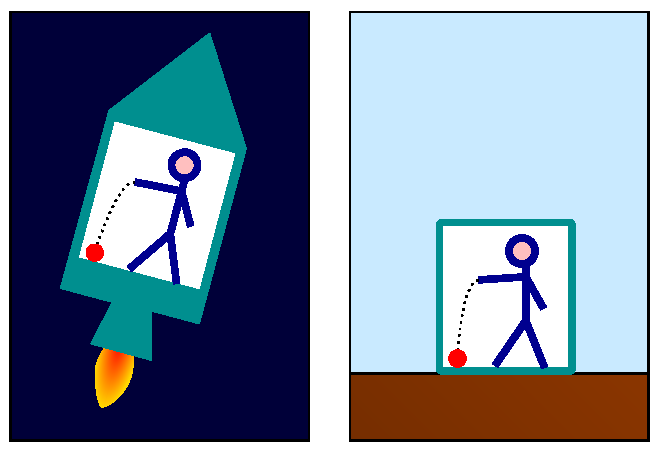
\includegraphics[width=0.7\textwidth]{figure/Elevator_gravity}
  \caption[Illustrazione sul principio di equivalenza]{A sinistra, razzo in moto
    accelerato nello spazio vuoto lontano dall'influenza di campo
    gravitazionali, a destra razzo fermo e sottoposto a un campo gravitazionale.
    {\footnotesize (Crediti: Markus Poessel e Pbroks13
      \url{https://commons.wikimedia.org/wiki/File:Elevator_gravity.svg})}}
  \label{fig:razzo-princ-equiv}
\end{figure}
Consideriamo ora le due situazioni rappresentate nella
figura~\ref{fig:razzo-princ-equiv}.  I corpi all'interno di un razzo che si
muove con accelerazione $\bm{a}=-\bm{g}$, lontano da qualsiasi altro campo
gravitazionale, sono soggetti a un'accelerazione $\bm{g}$ rispetto alle pareti.
L'osservatore non può quindi distinguere sperimentalmente questa situazione da
quella in cui in cui il razzo è fermo sulla Terra e soggetto al campo
gravitazionale planetario.  Nel razzo accelerato, una forza inerziale riproduce
lo stesso effetto della forza di gravità nel razzo a Terra.

Per quanto abbiamo visto, in una regione limitata dello spazio-tempo la forza di
gravità è indistinguibile da una forza inerziale e può essere cancellata o
simulata da quest'ultima.  Con un'opportuna trasformazione delle coordinate si
possono, allora, annullare localmente gli effetti del campo gravitazionale e il
sistema di riferimento apparirà, in questo modo, inerziale.  Einstein riassunse
tutte queste osservazioni in modo rigoroso nella formulazione forte del
\index{principio!di equivalenza!forte}\emph{principio di equivalenza}:
\emph{per ogni evento dello spazio-tempo in un arbitrario campo gravitazionale è
  possibile scegliere un sistema di riferimento \emph{localmente inerziale} (in
  caduta libera nel campo gravitazionale), tale che in un intorno
  sufficientemente piccolo dell'evento gli effetti della gravità siano assenti e
  le leggi della natura assumano la stessa forma che hanno in un sistema di
  riferimento inerziale}.
Dunque in un sistema di riferimento localmente inerziale la fisica segue le
leggi della relatività speciale.

% Vedi Hobson M., Efstathiou G., Lasenby A., "General relativity, An
% introduction for physicists", § 7.3, pagine 149-151.
Per rendere compatibili la teoria della relatività speciale e la gravitazione,
Einstein suggerì inoltre che la gravità non dovesse essere più considerata come
una forza, nel significato classico del termine, ma come una manifestazione
della curvatura dello spazio-tempo prodotta dalla presenza di materia.  In
assenza di campi gravitazionali la spazio-tempo è piatto e la metrica è quella
di Minkowski della relatività speciale.

\section{Equazione del moto di una particella in un campo gravitazionale}
\label{sec:equazione-moto}

Consideriamo una particella in caduta libera all'interno di un campo
gravitazionale.  In un sistema di riferimento, di coordinate $\xi^{\alpha}$,
localmente inerziale in cui la particella si muove di moto rettilineo uniforme
nello spazio-tempo, l'equazione del moto è
\begin{equation}
  \label{eq:moto-caduta-libera}
  \toder[2]{\xi^{\alpha}}{\tau} = 0,
\end{equation}
in cui $\dd \tau^{2} = -\eta_{\alpha\beta}\dd\xi^{\alpha}\dd\xi^{\beta}$ è
l'intervallo di tempo proprio.  Le coordinate $\xi^{\alpha}$ possono essere
espresse come funzione di un altro qualsiasi sistema di coordinate $x^{\mu}$ e
viceversa
\begin{align}
  \xi^{\alpha} &= \xi^{\alpha}(x^{\mu}), \\
  x^{\mu} &= x^{\mu}(\xi^{\alpha}).
\end{align}
% Poiché la trasformazione è invertibile deve risultare
% \begin{equation}
%   \abs*{\parder{x^{\mu}}{\xi^{\alpha}}} \neq 0.
% \end{equation}
Inoltre le coordinate $x^{\mu}$ dipendono anche dal tempo proprio $\tau$, allora
dalla~\eqref{eq:moto-caduta-libera} abbiamo
\begin{equation}
  \label{eq:moto1}
  0 = \toder{}{\tau}\toder{\xi^{\alpha}}{\tau} = \toder{}{\tau}
  \bigg( \parder{\xi^{\alpha}}{x^{\mu}}\toder{x^{\mu}}{\tau} \bigg)
  = \parder{\xi^{\alpha}}{x^{\mu},x^{\nu}} \toder{x^{\nu}}{\tau}
  \toder{x^{\mu}}{\tau} + \parder{\xi^{\alpha}}{x^{\mu}}
  \toder[2]{x^{\mu}}{\tau}.
\end{equation}
Supponendo che ciascuna delle quattro coordinate $x^{\mu}$ sia indipendente
dalle altre possiamo scrivere le relazioni
\begin{equation}
  \parder{x^{\lambda}}{x^{\mu}} = \tensor{\delta}{^{\lambda}_{\mu}}
  \implies \parder{x^{\lambda}}{\xi^{\alpha}} \parder{\xi^{\alpha}}{x^{\mu}} =
  \tensor{\delta}{^{\lambda}_{\mu}},
\end{equation}
quindi moltiplicando la~\eqref{eq:moto1} per
$\lparder{x^{\lambda}}{\xi^{\alpha}}$ l'equazione del moto diventa
\begin{equation}
  \tensor{\delta}{^{\lambda}_{\mu}} \toder[2]{x^{\mu}}{\tau} +
  \bigg(\parder{\xi^{\alpha}}{x^{\mu},x^{\nu}}\parder{x^{\lambda}}{\xi^{\alpha}}
  \bigg) \toder{x^{\mu}}{\tau} \toder{x^{\nu}}{\tau} = 0.
\end{equation}
Definendo la \index{connessione!affine}\emph{connessione affine}
$\tensor{\Gamma}{^{\lambda}_{\mu\nu}}$ come
\begin{equation}
  \label{eq:connessione-affine}
  \tensor{\Gamma}{^{\lambda}_{\mu\nu}}
  = \parder{\xi^{\alpha}}{x^{\mu},x^{\nu}} \parder{x^{\lambda}}{\xi^{\alpha}}
\end{equation}
l'equazione del moto può essere riscritta nel seguente modo
\begin{equation}
  \label{eq:geodetica}
  \toder[2]{x^{\lambda}}{\tau} + \tensor{\Gamma}{^{\lambda}_{\mu\nu}}
  \toder{x^{\mu}}{\tau} \toder{x^{\nu}}{\tau} = 0,
\end{equation}
oppure, utilizzando la quadrivelocità $u^{\alpha} = \ltoder{x^{\alpha}}{\tau}$,
\begin{equation}
  \label{eq:geodetica2}
  \toder{u^{\lambda}}{\tau} + \tensor{\Gamma}{^{\lambda}_{\mu\nu}}
  u^{\mu} u^{\nu} = 0.
\end{equation}
La~\eqref{eq:geodetica} è chiamata
\index{equazione!della geodetica}\emph{equazione della geodetica}.
$\tensor{\Gamma}{^{\lambda}_{\mu\nu}}$ è un insieme di $4^{3} = 64$ quantità che
tuttavia, come vedremo nel paragrafo~\ref{sec:connessione-affine}, \emph{non} si
trasformano, in generale, come un quadritensore di rango $3$.  Nonostante ciò è
utile indicarla con il simbolo di un tensore.  Dalla definizione di connessione
affine abbiamo inoltre che questa è simmetrica rispetto agli indici inferiori,
cioè
$\tensor{\Gamma}{^{\lambda}_{\mu\nu}} = \tensor{\Gamma}{^{\lambda}_{\nu\mu}}$.

L'intervallo di tempo proprio
$\dd\tau^{2} = -\eta_{\alpha\beta} \dd\xi^{\alpha} \dd\xi^{\beta}$ può essere
espresso rispetto alle coordinate $x^{\mu}$ come
\begin{equation}
  \begin{split}
    \dd\tau^{2} &= -\eta_{\alpha\beta} \parder{\xi^{\alpha}}{x^{\mu}}\dd
    x^{\mu} \parder{\xi^{\beta}}{x^{\nu}}\dd x^{\nu} \\
    &= -g_{\mu\nu}\dd x^{\mu}\dd x^{\nu},
  \end{split}
\end{equation}
dove
\begin{equation}
  \label{eq:tensore-metrico}
  g_{\mu\nu} =
  \eta_{\alpha\beta} \parder{\xi^{\alpha}}{x^{\mu}} \parder{\xi^{\beta}}{x^{\nu}}
\end{equation}
è il \index{tensore!metrico}\emph{tensore metrico}.  Il tensore metrico, a
differenza del tensore di Minkowski, in generale non è diagonale ed è funzione
delle coordinate poiché il valore delle derivate varia punto per punto.  Quindi
dovremmo scrivere $g_{\mu\nu}(x)$ ma per brevità ometteremo di specificare la
dipendenza dal punto.  Osserviamo che $g_{\mu\nu}$ è simmetrico rispetto allo
scambio degli indici in quanto il tensore metrico di Minkowski
$\eta_{\alpha\beta}$ è simmetrico, infatti
% NOTA: l'equazione seguente non è sbagliata: nel terzo membro si sfrutta la
% simmetria di \eta_{\mu\nu} e la commutatività del prodotto di due numeri,
% nello specifico delle due derivate parziali che sono state scambiate.
\begin{equation}
  g_{\nu\mu} =
  \eta_{\alpha\beta} \parder{\xi^{\alpha}}{x^{\nu}}\parder{\xi^{\beta}}{x^{\mu}}
  =
  \eta_{\beta\alpha} \parder{\xi^{\beta}}{x^{\mu}}\parder{\xi^{\alpha}}{x^{\nu}}
  = g_{\mu\nu}.
\end{equation}

Dall'equazione della geodetica risulta che il moto di una particella in un campo
gravitazionale è determinato dalla connessione affine.  Inoltre
$\ltoder{u^{\lambda}}{\tau}$ è la quadriaccelerazione del corpo, allora possiamo
interpretare la quantità
$-m\tensor{\Gamma}{^{\lambda}_{\mu\nu}} u^{\mu} u^{\nu}$ come la ``quadriforza''
agente sul corpo all'interno del campo gravitazionale.  Come vedremo nel
paragrafo~\ref{sec:relazione-g-Gamma}, le derivate di $g_{\mu\nu}$ definiscono
il campo $\tensor{\Gamma}{^{\lambda}_{\mu\nu}}$ e quindi il tensore metrico può
essere visto come il ``potenziale'' del campo gravitazionale.  In effetti nel
paragrafo~\ref{sec:limite-newtoniano} vedremo che nel limite newtoniano la
componente $g_{00}$ del tensore metrico è strettamente legata al potenziale
gravitazionale classico.  Chiaramente queste interpretazioni della connessione
affine e del tensore metrico sono solo un'analogia fisica derivante dal
confronto con le equazioni newtoniane del moto
$\bm{F} = m \bm{a} = - \nabla\phi$.

\section{Relazione fra tensore metrico e connessione affine}
\label{sec:relazione-g-Gamma}

Derivando rispetto a $x^{\lambda}$ l'espressione del tensore
metrico~\eqref{eq:tensore-metrico} abbiamo
\begin{equation}
  \partial_{\lambda}g_{\mu\nu}
  = \parder{\xi^{\alpha}}{x^{\lambda},x^{\mu}} \parder{\xi^{\beta}}{x^{\nu}}
  \eta_{\alpha\beta}
  + \parder{\xi^{\alpha}}{x^{\mu}} \parder{\xi^{\beta}}{x^{\lambda},x^{\nu}}
  \eta_{\alpha\beta}.
\end{equation}
Osserviamo che dalla definizione di connessione
affine~\eqref{eq:connessione-affine} risulta
\begin{equation}
  \parder{\xi^{\alpha}}{x^{\lambda}}\tensor{\Gamma}{^{\lambda}_{\mu\nu}}
  = \parder{\xi^{\alpha}}{x^{\mu},x^{\nu}},
\end{equation}
quindi
\begin{equation}
  \label{eq:foo}
  \begin{split}
    \partial_{\lambda}g_{\mu\nu} &=
    \tensor{\Gamma}{^{\rho}_{\lambda\mu}} \parder{\xi^{\alpha}}{x^{\rho}}
    \parder{\xi^{\beta}}{x^{\nu}} \eta_{\alpha\beta} +
    \tensor{\Gamma}{^{\rho}_{\lambda\nu}} \parder{\xi^{\alpha}}{x^{\mu}}
    \parder{\xi^{\beta}}{x^{\rho}}
    \eta_{\alpha\beta} \\
    &= \tensor{\Gamma}{^{\rho}_{\lambda\mu}}g_{\rho\nu} +
    \tensor{\Gamma}{^{\rho}_{\lambda\nu}}g_{\rho\mu}.
  \end{split}
\end{equation}
Calcolando in maniera $\partial_{\mu}g_{\lambda\nu}$ e
$\partial_{\nu}g_{\mu\lambda}$ si giunge all'equazione
\begin{equation}
  \begin{split}
    \partial_{\lambda}g_{\mu\nu} + \partial_{\mu}g_{\lambda\nu}
    - \partial_{\nu}g_{\mu\lambda} &=
    \tensor{\Gamma}{^{\rho}_{\lambda\mu}}g_{\rho\nu} +
    \tensor{\Gamma}{^{\rho}_{\lambda\nu}}g_{\rho\mu} +
    \tensor{\Gamma}{^{\rho}_{\mu\lambda}}g_{\rho\nu} +
    \tensor{\Gamma}{^{\rho}_{\mu\nu}}g_{\rho\lambda} \\
    &- \tensor{\Gamma}{^{\rho}_{\nu\mu}}g_{\rho\lambda} -
    \tensor{\Gamma}{^{\rho}_{\nu\lambda}}g_{\rho\mu} \\
    &= 2g_{\rho\nu} \tensor{\Gamma}{^{\rho}_{\lambda\mu}},
  \end{split}
\end{equation}
avendo ricordato che $g_{\mu\nu}$ e $\tensor{\Gamma}{^{\rho}_{\mu\nu}}$ sono
simmetrici per scambi degli indici $\mu$ e $\nu$.  Definiamo la matrice
$g^{\nu\sigma}$ come l'inversa di $g_{\nu\sigma}$, cioè
$g^{\nu\sigma}g_{\rho\nu} = \tensor{\delta}{^{\sigma}_{\rho}}$, allora,
moltiplicando primo e ultimo membro dell'equazione precedente per
$g^{\nu\sigma}$
\begin{equation}
  g^{\nu\sigma}(\partial_{\lambda}g_{\mu\nu} + \partial_{\mu}g_{\lambda\nu}
  - \partial_{\nu}g_{\mu\lambda}) = 2\tensor{\Gamma}{^{\sigma}_{\lambda\mu}}
\end{equation}
otteniamo la seguente relazione fra il \index{tensore!metrico}tensore metrico e
la \index{connessione!affine}connessione
affine\footnote{Presentiamo un utile metodo per ricordare la relazione fra
  tensore metrico e connessione affine.  Osservando che il tensore metrico è
  simmetrico, la connessione affine è simmetrica nei suoi due indici inferiori e
  che nella relazione compaiono due derivate con il segno $+$ e una con il segno
  $-$ deduciamo che nell'unica derivata con il segno $-$ il tensore metrico deve
  avere gli stessi indici inferiori della connessione affine e la derivata è
  fatta rispetto all'indice muto, nelle derivate con il segno $+$ il tensore
  metrico ha sempre uno degli indici uguale all'indice muto e l'altro uguale a
  uno degli indici inferiori della connessione affine mentre la derivata è fatta
  rispetto all'altro indice inferiore della connessione affine.  Infine, il
  tensore metrico controvariante che compare davanti alle parentesi avrà un
  indice uguale all'unico indice superiore della connessione affine e l'altro
  uguale all'indice muto.}
\begin{equation}
  \label{eq:connessione-metrica}
  \tensor{\Gamma}{^{\sigma}_{\lambda\mu}} =
  \frac{1}{2} g^{\nu\sigma} (\partial_{\lambda}g_{\mu\nu}
  + \partial_{\mu}g_{\lambda\nu} - \partial_{\nu}g_{\lambda\mu}).
\end{equation}

L'equazione della geodetica~\eqref{eq:geodetica} per una particella in caduta
libera può essere ricavata applicando il principio variazionale alla distanza
$S$ fra due eventi $A$ e $B$ nello spazio-tempo
\begin{equation}
  S = \int_{A}^{B} \dd\tau.
\end{equation}
Conviene parametrizzare la linea d'universo $x^{\mu}$ della particella con un
arbitrario parametro $p$, cioè $x^{\mu} = x^{\mu}(p)$, quindi
\begin{equation}
  S = \int_{A}^{B} \dd\tau = \int_{A}^{B} \toder{\tau}{p}\dd p =
  \int_{A}^{B} \bigg( -g_{\mu\nu}\toder{x^{\mu}}{p}\toder{x^{\nu}}{p}
  \bigg)^{1/2} \dd p.
\end{equation}
Per ricavare l'equazione del moto dobbiamo imporre che $S$ sia stazionario
rispetto a variazioni infinitesime $\delta x^{\mu}$ delle coordinate $x^{\mu}$,
con la condizione che le variazioni sia nulle nei punti $A$ e $B$
\begin{equation}
  \label{eq:condizione-variazione}
  \delta x_{A}^{\mu} = \delta x_{B}^{\mu} = 0.
\end{equation}
La variazione della distanza fra i due eventi è
\begin{equation}
  \begin{split}
    \delta S &= \int_{A}^{B} \frac{1}{2}\bigg( -g_{\mu\nu} \toder{x^{\mu}}{p}
    \toder{x^{\nu}}{p} \bigg)^{-1/2} \bigg( -\parder{g_{\mu\nu}}{x^{\lambda}}
    \delta x^{\lambda} \toder{x^{\mu}}{p} \toder{x^{\nu}}{p} \\
    &- g_{\mu\nu} \toder{\delta x^{\mu}}{p} \toder{x^{\nu}}{p} - g_{\mu\nu}
    \toder{x^{\mu}}{p} \toder{\delta x^{\nu}}{p} \bigg) \dd p \\
    &= \int_{A}^{B} \frac{1}{2}\bigg( -g_{\mu\nu} \toder{x^{\mu}}{p}
    \toder{x^{\nu}}{p} \bigg)^{-1/2} \bigg( -\parder{g_{\mu\nu}}{x^{\lambda}}
    \delta x^{\lambda} \toder{x^{\mu}}{p} \toder{x^{\nu}}{p} -
    2g_{\mu\nu}\toder{\delta x^{\mu}}{p} \toder{x^{\nu}}{p} \bigg) \dd p.
  \end{split}
\end{equation}
Nell'ultimo passaggio abbiamo sfruttato la simmetria del tensore metrico
$g_{\mu\nu}$.  Osserviamo che il primo fattore dell'integrale è
$\ltoder{p}{\tau}$, così che risulta
\begin{equation}
  \delta S = -\int_{A}^{B} \bigg( \frac{1}{2}\parder{g_{\mu\nu}}{x^{\lambda}}
  \delta  x^{\lambda} \toder{x^{\mu}}{\tau} \toder{x^{\nu}}{\tau} + g_{\mu\nu}
  \toder{\delta x^{\mu}}{\tau} \toder{x^{\nu}}{\tau} \bigg) \dd \tau.
\end{equation}
Integriamo il secondo termine per parti ricordando la
condizione~\eqref{eq:condizione-variazione}
\begin{equation}
  \begin{split}
    \int_{A}^{B} g_{\lambda\nu} \toder{\delta x^{\lambda}}{\tau}
    \toder{x^{\nu}}{\tau} \dd \tau &= \bigg[g_{\lambda\nu} \delta x^{\lambda}
    \toder{x^{\nu}}{\tau} \bigg]_{A}^{B} - \int_{A}^{B} \delta x^{\lambda}
    \toder{}{\tau} \bigg( g_{\lambda\nu} \toder{x^{\nu}}{\tau} \bigg) \dd\tau \\
    &= -\int_{A}^{B} \delta x^{\lambda} \bigg( \toder{g_{\lambda\nu}}{\tau}
    \toder{x^{\nu}}{\tau} + g_{\lambda\nu}\toder[2]{x^{\nu}}{\tau} \bigg) \dd
    \tau \\
    &= -\int_{A}^{B} \delta x^{\lambda}
    \bigg( \parder{g_{\lambda\nu}}{x^{\mu}} \toder{x^{\mu}}{\tau}
    \toder{x^{\nu}}{\tau} + g_{\lambda\nu}\toder[2]{x^{\nu}}{\tau} \bigg) \dd
    \tau.
  \end{split}
\end{equation}
Allora
\begin{equation}
  \delta S = -\int_{A}^{B} \delta x^{\lambda} \bigg(
  \frac{1}{2} \parder{g_{\mu\nu}}{x^{\lambda}} \toder{x^{\mu}}{\tau}
  \toder{x^{\nu}}{\tau} - \parder{g_{\lambda\nu}}{x^{\mu}}
  \toder{x^{\mu}}{\tau} \toder{x^{\nu}}{\tau} -
  g_{\lambda\nu}\toder[2]{x^{\nu}}{\tau} \bigg) \dd \tau.
\end{equation}
Affinché sia $\delta S = 0$, per l'arbitrarietà della variazione
$\delta x^{\lambda}$ deve annullarsi la quantità fra parentesi, cioè
\begin{equation}
  \bigg(\frac{1}{2} \partial_{\lambda} g_{\mu\nu} - \partial_{\mu}g_{\lambda\nu}
  \bigg) \toder{x^{\mu}}{\tau} \toder{x^{\nu}}{\tau}
  - g_{\lambda\nu}\toder[2]{x^{\nu}}{\tau} = 0.
\end{equation}
Sfruttando il fatto che gli indici muti possono essere scambiati possiamo
scrivere
\begin{equation}
  \partial_{\mu}g_{\lambda\nu} \toder{x^{\mu}}{\tau} \toder{x^{\nu}}{\tau} =
  \frac{1}{2} (\partial_{\mu}g_{\lambda\nu} + \partial_{\nu}g_{\lambda\mu})
  \toder{x^{\mu}}{\tau} \toder{x^{\nu}}{\tau},
\end{equation}
quindi
\begin{equation}
  \frac{1}{2} (\partial_{\lambda} g_{\mu\nu} - \partial_{\mu}g_{\lambda\nu}
  - \partial_{\nu}g_{\lambda\mu}) \toder{x^{\mu}}{\tau}
  \toder{x^{\nu}}{\tau} - g_{\lambda\nu}\toder[2]{x^{\nu}}{\tau} = 0
\end{equation}
e poiché
$(\partial_{\lambda} g_{\mu\nu} - \partial_{\mu}g_{\lambda\nu}
- \partial_{\nu}g_{\lambda\mu})/2 = -g_{\rho\lambda}
\tensor{\Gamma}{^{\rho}_{\nu\mu}}$ abbiamo
\begin{equation}
  g_{\rho\lambda} \tensor{\Gamma}{^{\rho}_{\nu\mu}} \toder{x^{\mu}}{\tau}
  \toder{x^{\nu}}{\tau} + g_{\lambda\nu}\toder[2]{x^{\nu}}{\tau} = 0.
\end{equation}
Moltiplicando infine ambo i membri per $g^{\lambda\sigma}$ e ricordando che
$g_{\alpha\beta}g^{\alpha\gamma} = \tensor{\delta}{^{\gamma}_{\beta}}$ giungiamo
all'\index{equazione!della geodetica}equazione della geodetica
\begin{equation}
  \toder[2]{x^{\sigma}}{\tau} + \tensor{\Gamma}{^{\sigma}_{\nu\mu}}
  \toder{x^{\mu}}{\tau} \toder{x^{\nu}}{\tau} = 0.
\end{equation}
Poiché abbiamo ricavato questa equazione determinando il percorso che deve
seguire un corpo in caduta libera in un campo gravitazionale in maniera tale che
la distanza percorsa sia un estremo (e in particolare si tratta spesso di un
minimo), possiamo dare un'interpretazione geometrica \emph{a posteriori}
dell'equazione del moto: un corpo in caduta libera all'interno di un campo
gravitazionale si muoverà lungo un percorso il più breve (o lungo) possibile fra
due eventi nello spazio-tempo deformato dalla presenza del campo e la distanza è
misurata dal tempo proprio.  Un percorso simile è chiamato \emph{geodetica}, da
cui il nome dell'equazione~\eqref{eq:geodetica}.

\section{Limite newtoniano dell'equazione del moto}
\label{sec:limite-newtoniano}

Vogliamo vedere come l'equazione del moto~\eqref{eq:geodetica} di una particella
all'interno di un campo gravitazionale si riduce considerando il limite
newtoniano, vale a dire nelle condizioni
\begin{itemize}
\item il campo gravitazionale è debole, cioè può essere considerato come una
  perturbazione dello spazio-tempo piatto;
\item il campo gravitazionale inoltre è stazionario;
\item la velocità della particella è molto più piccola di quella della luce.
\end{itemize}
La prima condizione può essere formalizzata dicendo che il
\index{tensore!metrico}tensore metrico $g_{\mu\nu}$ deve differire di poco dal
tensore di Minkowski dello spazio-tempo piatto
\begin{equation}
  g_{\mu\nu} = \eta_{\mu\nu} + h_{\mu\nu},
\end{equation}
in cui $\abs{h_{\mu\nu}} \ll 1$ sono piccole correzioni che determinano il campo
gravitazionale.  Poiché sia $g_{\mu\nu}$ sia $\eta_{\mu\nu}$ sono simmetrici
nello scambio degli indici, tale dovrà essere anche $h_{\mu\nu}$.  Osserviamo
che
\begin{equation}
  \tensor{h}{^{\mu}_{\nu}} = g_{\nu\lambda}h^{\mu\lambda} =
  \eta_{\nu\lambda}h^{\mu\lambda} + h_{\nu\lambda}h^{\mu\lambda} =
  \eta_{\nu\lambda}h^{\mu\lambda} + \mathcal{O}(h^{2}),
\end{equation}
cioè al primo ordine della perturbazione della metrica le operazioni di
innalzamento e abbassamento degli indici di $h_{\mu\nu}$ vengono eseguite con il
tensore metrico non perturbato $\eta_{\mu\nu}$ invece che con il tensore metrico
``completo'' $g_{\mu\nu}$.  Nel seguito, trattando campi deboli in cui la
metrica è approssimabile con $g_{\mu\nu} = \eta_{\mu\nu} + h_{\mu\nu}$,
seguiremo sempre questa convenzione.  Inoltre la correzione al primo ordine
negli infinitesimi per il tensore metrico controvariante è data da (vedi
l'appendice~\ref{sec:dimostr-correz-metrica-controvariante})
\begin{equation}
  \label{eq:correzione-metrica-controvariante}
  g^{\mu\nu} = \eta^{\mu\nu} - h^{\mu\nu},
\end{equation}
dove $h^{\mu\nu} = \eta^{\mu\lambda}\eta^{\nu\sigma} h_{\lambda\sigma}$.
Calcoliamo la connessione affine al primo ordine della perturbazione
$h_{\mu\nu}$
\begin{equation}
  \label{eq:christoffel-approx}
  \tensor{\Gamma}{^{\sigma}_{\mu\nu}} = \frac{1}{2}g^{\lambda\sigma}
  (\partial_{\mu}g_{\nu\lambda} + \partial_{\nu}g_{\mu\lambda}
  - \partial_{\lambda}g_{\mu\nu}) \approx \frac{1}{2}\eta^{\lambda\sigma}
  (\partial_{\mu}h_{\nu\lambda} + \partial_{\nu}h_{\mu\lambda}
  - \partial_{\lambda}h_{\mu\nu}).
\end{equation}
Nel paragrafo~\ref{sec:equazione-moto} abbiamo interpretato il tensore metrico
come il potenziale gravitazionale.  Nello studio del limite newtoniano
$h_{\mu\nu}$ rappresenta la deviazione rispetto al caso di assenza di gravità
($g_{\mu\nu} = \eta_{\mu\nu}$), quindi ci aspettiamo che il potenziale
gravitazionale newtoniano sia contenuto interamente in questo termine.

La terza condizione può essere formalizzata come
\begin{equation}
  \toder{x^{i}}{\tau} \ll \toder{t}{\tau},
\end{equation}
e l'equazione della geodetica si riduce a
\begin{equation}
  \label{eq:geodetica-approx}
  \begin{split}
    0 &= \toder[2]{x^{\sigma}}{\tau} + \tensor{\Gamma}{^{\sigma}_{\lambda\mu}}
    \toder{x^{\lambda}}{\tau} \toder{x^{\mu}}{\tau} \\
    &= \toder[2]{x^{\sigma}}{\tau} + \tensor{\Gamma}{^{\sigma}_{00}} \bigg(
    \toder{t}{\tau} \bigg)^{2} + 2\tensor{\Gamma}{^{\sigma}_{0i}}\toder{t}{\tau}
    \toder{x^{i}}{\tau} + \tensor{\Gamma}{^{\sigma}_{ij}} \toder{x^{i}}{\tau}
    \toder{x^{j}}{\tau} \\
    &\approx \toder[2]{x^{\sigma}}{\tau} + \tensor{\Gamma}{^{\sigma}_{00}}\bigg(
    \toder{t}{\tau} \bigg)^{2}.
  \end{split}
\end{equation}
Dalla~\eqref{eq:christoffel-approx} risulta
\begin{equation}
  \tensor{\Gamma}{^{\sigma}_{00}} \approx
  \frac{1}{2}\eta^{\lambda\sigma}(\partial_{0}h_{0\lambda}
  + \partial_{0}h_{0\lambda} - \partial_{\lambda}h_{00}) =
  -\frac{1}{2}\eta^{\lambda\sigma} \partial_{\lambda}h_{00},
\end{equation}
in quanto le derivate temporali di $h_{\mu\nu}$ sono nulle in base alla seconda
condizione che descrive il limite newtoniano.  Notiamo che per $\sigma=0$ si ha
$\tensor{\Gamma}{^{0}_{00}}=0$.  Allora la~\eqref{eq:geodetica-approx}
corrisponde, al variare di $\sigma$, alle equazioni
\begin{subequations}
  \begin{align}
    \toder[2]{t}{\tau} &= 0 &\text{per $\sigma = 0$}, \\
    \toder[2]{x^{i}}{\tau} &= \frac{1}{2} \bigg( \toder{t}{\tau} \bigg)^{2}
    (\nabla h_{00})_{i} &\text{per $\sigma = i$}.
  \end{align}
\end{subequations}
La prima equazione ci dice che $\ltoder{t}{\tau}$ è una costante, mentre dalla
seconda, dividendo per $(\ltoder{t}{\tau})^{2}$, abbiamo
\begin{equation}
  \toder[2]{\bm{x}}{t} = \frac{1}{2}\nabla h_{00}.
\end{equation}
L'equazione newtoniana del moto è
\begin{equation}
  \bm{a}_{\textup{N}} = \toder[2]{\bm{x}}{t} = -\nabla\phi,
\end{equation}
in cui $\phi$ è il potenziale newtoniano del campo gravitazionale, legato alla
distribuzione di massa $\rho$
\index{equazione!di Poisson!per il campo gravitazionale}dall'equazione di
Poisson $\nabla^{2} \phi = 4\pi G\rho$.  Confrontando le due equazioni
precedenti troviamo
\begin{equation}
  h_{00} = -2\phi + \text{costante}.
\end{equation}
A grandi distanze dal corpo, cioè nel limite $r \to \infty$, il potenziale
newtoniano $\phi$ si annulla, il campo gravitazionale è assente e il tensore
metrico $g_{\mu\nu}$ deve tendere al tensore di Minkowski $\eta_{\mu\nu}$ dello
spazio-tempo piatto, cioè si devono annullare tutte le componenti di
$h_{\mu\nu}$.  Pertanto ricaviamo che la costante deve essere uguale a $0$ e
$h_{00} = -2\phi$ o, ripristinando la velocità $c$ della luce nel vuoto,
$h_{00} = -2\phi/c^{2}$.  Nel caso particolare di un campo gravitazionale
prodotto da un corpo sferico di massa $M$ e raggio $R$, l'espressione del
potenziale a distanza $r > R$ è $\phi = -GM/r$, quindi
\begin{equation}
  \label{eq:h00}
  h_{00} = -\frac{2\phi}{c^{2}} = \frac{2GM}{rc^{2}} = \frac{r_{\textup{S}}}{r},
\end{equation}
in cui
\begin{equation}
  r_{\textup{S}} = \frac{2GM}{c^{2}}
\end{equation}
è il \index{raggio!di Schwarzschild}\emph{raggio di Schwarzschild} del corpo che
genera il campo gravitazionale.  Dunque abbiamo trovato che $h_{00}$ è
esattamente il potenziale gravitazionale newtoniano a meno di fattori
moltiplicativi costanti, coerentemente con quanto previsto all'inizio della
discussione del problema.  La componente $g_{00}$ del tensore metrico è
\begin{equation}
  g_{00} = \eta_{00} + h_{00} = -\bigg(1 + \frac{2\phi}{c^{2}}\bigg) = -
  \bigg(1 - \frac{2GM}{rc^{2}} \bigg).
\end{equation}
Poiché abbiamo ottenuto questi risultati nell'ipotesi di campo debole, cioè
$\abs{h_{\mu\nu}} \ll 1$, la quantità $h_{00} = -2\phi/c^{2} = r_{\textup{S}}/r$
dà una misura delle deviazioni della relatività generale rispetto alle
previsioni della fisica newtoniana.

\begin{table}
  \centering
  \caption[Valori del raggio di Schwarzschild per diversi corpi]{Valori del
    raggio di Schwarzschild $r_{\textup{S}}$ per diversi oggetti e valore della
    correzione $r_{\textup{S}}/r$ sulla superficie dei corpi.  $r$ è il raggio
    degli oggetti.  Questi valori sono approssimativi, sono rilevanti gli ordini
    di grandezza}
  \label{tab:Schwarzschild}
  \begin{tabular}{lSSSS}
    \toprule
    corpo & {$r_{\textup{S}}$ (\si{\metre})} & {$r$ (\si{\metre})} &
    {$r_{\textup{S}}/r$} \\
    \midrule
    Terra                     & 8.7e-3 & 6.4e6 & 1.4e-9 \\
    Sole                      & 3e3    & 7e8   & 4.3e-6 \\
    nana bianca               & 3e3    & 1e6   & 3e-3   \\
    stella di neutroni        & 3e3    & 1e4   & 0.3    \\
    buco nero di massa solare & 3e4    & 3e4   & 1      \\
    \bottomrule
  \end{tabular}
\end{table}
Nella tabella~\ref{tab:Schwarzschild} sono riportati i valori delle deviazioni
$r_{\textup{S}}/r$ dalla gravitazione newtoniana sulla superficie di alcuni
corpi.  Mentre per la Terra, il Sole e le nane bianche queste correzioni sono
generalmente piccole, non è possibile descrivere le vicinanze di corpi come le
stelle di neutroni o i buchi neri utilizzando la fisica newtoniana ma bisogna
tenere necessariamente in considerazione la relatività generale.  Tuttavia anche
per quanto riguarda il Sole e i pianeti del sistema solare sono osservati
effetti di relatività generale non previsti dalla teoria newtoniana, come
l'effetto Lense-Thirring, la dilatazione del tempo e il redshift gravitazionali,
la precessione del perielio e la deflessione della luce.

\section{Campo gravitomagnetico}
\label{sec:campo-gravitomagnetico}

Nella teoria newtoniana della gravitazione la velocità di una particella in
orbita attorno a un corpo di massa $M$ a distanza $r$ è data, per il teorema del
viriale $2K = -U \iff mv^{2} = GMm/r$, da $v = \sqrt{GM/r}$.  Nel paragrafo
precedente abbiamo studiato l'equazione del moto sotto le ipotesi di campo
debole ($\abs{h_{\mu\nu}} \sim GM/r \sim v^{2} \ll 1$), statico e velocità non
relativistiche ($v \ll 1$) trascurando i termini dell'ordine di
$\abs{h_{\mu\nu}}v^{2} \sim v^{4}$ e $\abs{h_{\mu\nu}}v \sim v^{3}$.  In questo
paragrafo studieremo l'equazione della geodetica con un livello di
approssimazione minore: continueremo a trascurare i termini dell'ordine di
$\abs{h_{\mu\nu}}v^{2}$ ma non quelli dell'ordine di $\abs{h_{\mu\nu}}v$.

Nelle ipotesi illustrate, le componenti $k$ dell'equazione della
geodetica~\eqref{eq:geodetica} sono date da
\begin{equation}
    \begin{split}
    0 &= \toder[2]{x^{k}}{\tau} + \tensor{\Gamma}{^{k}_{\lambda\mu}}
    \toder{x^{\lambda}}{\tau} \toder{x^{\mu}}{\tau} \\
    &= \toder[2]{x^{k}}{\tau} + \tensor{\Gamma}{^{k}_{00}} \bigg(
    \toder{t}{\tau} \bigg)^{2} + 2\tensor{\Gamma}{^{k}_{0i}}\toder{t}{\tau}
    \toder{x^{i}}{\tau} + \tensor{\Gamma}{^{k}_{ij}} \toder{x^{i}}{\tau}
    \toder{x^{j}}{\tau} \\
    &\approx \toder[2]{x^{k}}{\tau} + \tensor{\Gamma}{^{k}_{00}}\bigg(
    \toder{t}{\tau} \bigg)^{2} + 2\tensor{\Gamma}{^{k}_{0i}}\toder{t}{\tau}
    \toder{x^{i}}{\tau}.
  \end{split}
\end{equation}
Poiché stiamo ancora considerando velocità non relativistiche poniamo
$\dd \tau \approx \dd t$ e
$\ltoder{x^{k}}{\tau} \approx \ltoder{x^{k}}{t} = v^{k}$
\begin{equation}
  \label{eq:gem1}
  \toder{v^{k}}{t} + \tensor{\Gamma}{^{k}_{00}} +
  2\tensor{\Gamma}{^{k}_{0i}}v^{i} = 0.
\end{equation}
Ricordando che stiamo trattando campi gravitazionali statici, le componenti
della connessione affine che ci servono sono
\begin{subequations}
  \begin{align}
    \tensor{\Gamma}{^{k}_{00}} &=
    \frac{1}{2}\eta^{k\sigma}(\partial_{0}h_{0\sigma} + \partial_{0}h_{0\sigma}
    - \partial_{\sigma}h_{00}) = - \frac{1}{2}\partial^{k}h_{00}, \\
    \tensor{\Gamma}{^{k}_{0i}} &= \tensor{\Gamma}{^{k}_{i0}} =
    \frac{1}{2}\eta^{k\sigma} (\partial_{0}h_{i\sigma} + \partial_{i}h_{0\sigma}
    - \partial_{\sigma}h_{0i}) = \frac{1}{2}(\partial_{i}\tensor{h}{_{0}^{k}}
    - \partial^{k}h_{0i}).
  \end{align}
\end{subequations}
Abbassando gli indici liberi nell'equazione~\eqref{eq:gem1} così abbiamo
\begin{equation}
  \label{eq:gem2}
  \toder{v_{k}}{t} = \frac{1}{2}\partial_{k}h_{00} + (\partial_{k}h_{0i}
  - \partial_{i}h_{0k})v^{i}.
\end{equation}
Definiamo la matrice $4 \times 4$ antisimmetrica di componenti $f_{\alpha\beta}$
date da
\begin{equation}
  f_{\alpha\beta} = \frac{1}{2}(h_{0\beta,\alpha} - h_{0\alpha,\beta}) =
  -f_{\beta\alpha}.
\end{equation}
Osserviamo che non si tratta di un vero tensore di rango $2$ perché questa
quantità si trasforma come le componenti $0\alpha\beta$ di un tensore di rango
$3$.  Definiamo il vettore tridimensionale $\bm{g}$ di componenti
\begin{equation}
  g_{k} = -f_{0k} = \frac{1}{2}h_{00,k} = \frac{1}{2}(\nabla h_{00})_{k} =
  -(\nabla \phi)_{k},
\end{equation}
in cui abbiamo ricordato il risultato $h_{00} = -2\phi$ trovato nel paragrafo
precedente.  Osserviamo che $\bm{g} = -\nabla \phi$, quindi $\bm{g}$ è proprio
il campo gravitazionale newtoniano.  Con queste posizioni l'equazione della
geodetica~\eqref{eq:gem2} diventa
\begin{equation}
  \label{eq:gem3}
  \toder{v_{k}}{t} = g_{k} + 2f_{ki}v^{i}.
\end{equation}

Inoltre definiamo il vettore
tridimensionale $\bm{b}$ di componenti
\begin{subequations}
  \begin{align}
    b_{1} &= b_{x} = h_{03,2} - h_{02,3} = -2f_{32} = 2f_{23}, \\
    b_{2} &= b_{y} = h_{01,3} - h_{03,1} = -2f_{13} = 2f_{31}, \\
    b_{3} &= b_{z} = h_{02,1} - h_{01,2} = -2f_{21} = 2f_{12}.
  \end{align}
\end{subequations}
In maniera più compatta possiamo indicare ciascuna componente del vettore
$\bm{b}$ con (si somma su $j$ e $k$)
\begin{equation}
  b_{i} = \epsilon_{ijk}h_{0k,j} = \epsilon_{ijk}\partial_{j}h_{k},
\end{equation}
dove $\epsilon^{ijk}$ è il simbolo di Levi-Civita tridimensionale e abbiamo
definito il vettore tridimensionale
$\bm{h} = (h_{1}, h_{2}, h_{3}) = (h_{01}, h_{02}, h_{03})$.  Questo ci permette
di scrivere $\bm{b}$ come il rotore di $\bm{h}$
\begin{equation}
  \bm{b} = \nabla \times \bm{h}.
\end{equation}
La matrice $f_{\alpha\beta}$ è allora data da
\begin{equation}
  f_{\alpha\beta} =
  \begin{pmatrix}
    0     & -g_{x}   & -g_{y}   & -g_{z}   \\
    g_{x} & 0        & b_{z}/2  & -b_{y}/2 \\
    g_{y} & -b_{z}/2 & 0        & b_{x}/2  \\
    g_{z} & b_{y}/2  & -b_{x}/2 & 0
  \end{pmatrix}.
\end{equation}
Questa matrice è molto simile al tensore
elettromagnetico~\eqref{eq:tensore-elettromagnetico},\footnote{Abbiamo definito
  i vettori $\bm{g}$ e $\bm{b}$ con i segni opposti rispetto a quelli
  di~\textcite[138-139]{ohanian:gravitazione} solo al fine di avere gli stessi
  segni nella matrice $f_{\alpha\beta}$ e nel tensore elettromagnetico.  È una
  scelta di pura convenienza e non influisce sui risultati fisici
  successivi.\label{nota-b}} con il campo gravitazionale newtoniano $\bm{g}$ che
svolge il ruolo del campo elettrico $\bm{E}$ e $\bm{b}/2$ quello del campo
magnetico $\bm{B}$.  Data questa similitudine, $\bm{b}$ viene chiamato
\emph{campo gravitomagnetico}.  Una sfera carica ferma genera solo un campo
elettrico, una sfera in rotazione genera anche un campo magnetico.  In analogia,
ci aspettiamo che una massa rotante generi un campo gravitomagnetico non nullo.
Nel prossimo paragrafo scopriremo che questa intuizione è corretta.

Il parallelo con il campo elettromagnetico non si ferma qui.  Innanzitutto
notiamo che
\begin{equation}
  \begin{split}
    \epsilon_{kij}b^{j} &= \epsilon_{kij}\epsilon^{jlm}h_{0m,l} =
    -\epsilon_{jik}\epsilon^{jlm} h_{0m,l} = (\tensor{\delta}{_{i}^{m}}
    \tensor{\delta}{_{k}^{l}} - \tensor{\delta}{_{i}^{l}}
    \tensor{\delta}{_{k}^{m}}) h_{0m,l} = h_{0i,k} - h_{0k,i} \\
    &= 2f_{ki}.
  \end{split}
\end{equation}
Quindi la componente $k$ del prodotto vettoriale fra il vettore velocità
$\bm{v}$ e il campo gravitomagnetico $\bm{b}$ è
\begin{equation}
  (\bm{v}\times\bm{b})_{k} = \epsilon_{kij}v^{i}b^{j} = 2f_{ki}v^{i}.
\end{equation}
Allora possiamo scrivere l'equazione della geodetica~\eqref{eq:gem3} nella
seguente forma vettoriale
\begin{equation}
  \toder{\bm{v}}{t} = \bm{g} + \bm{v}\times\bm{b}.
\end{equation}
Quindi $\bm{g}$ e $\bm{b}$ soddisfano un'equazione analoga
alla~\eqref{eq:forza-lorentz} soddisfatta della forza di Lorentz.  Inoltre
usando la definizione di $f_{\alpha\beta}$ si verifica che risulta
\begin{equation}
  f_{\alpha\beta,\gamma} + f_{\gamma\alpha,\beta} + f_{\beta\gamma,\alpha} = 0,
\end{equation}
che è un'equazione analoga all'equazione di Maxwell senza
sorgenti~\eqref{eq:maxwell-cov22}.  Poiché questa equazione è equivalente alle
equazioni $\nabla \cdot \bm{B} = 0$ e
$\nabla\times\bm{E} = - \lparder{\bm{B}}{t}$, deduciamo immediatamente che per
$\bm{g}$ e $\bm{b}$ deve inoltre risultare
\begin{subequations}
  \begin{align}
    \nabla \cdot \bm{b} &= 0, \\
    \nabla\times\bm{g} &= -\frac{1}{2}\parder{\bm{b}}{t}.
  \end{align}
\end{subequations}
Nel limite newtoniano il potenziale gravitazionale $\phi$ soddisfa
\index{equazione!di Poisson!per il campo gravitazionale}l'equazione di Poisson
$\nabla^{2} \phi = 4\pi G \rho$, quindi ricordando che $\bm{g} = -\nabla \phi$
otteniamo l'ulteriore relazione
\begin{equation}
  \nabla \cdot \bm{g} = -4\pi G \rho.
\end{equation}
Per trovare l'ultima ``equazione di Maxwell'' per il campo gravitomagnetico
dobbiamo sfruttare la seguente equazione valida per un campo gravitazionale
debole e indipendente dal tempo
% Nota: il segno del laplaciano nell'equazione [3.121] dell'Ohanian-Ruffini (a
% pagina 139 nell'edizione italiana) è diverso per la diversa scelta dei segni
% della metrica che comporta un segno opposto nel dalambertiano.
\begin{equation}
  \nabla^{2}h^{0k} - \partial_{l}\partial^{k} h^{0l} = \partial_{l}\partial^{l}
  h^{0k} - \partial_{l}\partial^{k} h^{0l} = -16\pi GT^{0k},
\end{equation}
in cui $T^{0k} = \rho v^{k}$ è la componente $0k$ del tensore energia-impulso,
quindi rappresenta la densità di flusso di energia nella direzione $k$.  Questa
equazione deriva dall'approssimazione lineare delle equazioni di
Einstein\footnote{Anticipiamo che l'equazione precedente può essere ricavata
  inserendo nelle componenti $0k$ dell'equazione di
  Einstein~\eqref{eq:einstein-lineare-esatta} l'approssimazione lineare del
  tensore di Ricci~\eqref{eq:ricci-lineare}, con l'ipotesi di campo statico,
  cioè le cui derivate temporali sono nulle.}  e può anche essere scritta come
\begin{equation}
  -16\pi GT^{0k} = \partial_{l}(h^{0k,l} - h^{0l,k}) = 2\partial_{l}f^{lk} =
  \epsilon^{lkj}\partial_{l}b_{j} = -\epsilon^{klj}\partial_{l}b_{j} = -(\nabla
  \times \bm{b})^{k},
\end{equation}
oppure nella seguente forma vettoriale
\begin{equation}
  \nabla \times \bm{b} = 16\pi G \bm{S},
\end{equation}
in cui $\bm{S} = (T^{01}, T^{02}, T^{03}) = \rho \bm{v}$ è l'analogo del
\index{vettore!di Poynting}vettore di Poynting $\bm{E}\times\bm{B}/4\pi$ per il
campo gravitomagnetico.

\subsection{Effetto Lense-Thirring}
\label{sec:effetto-lense-thirring}

Ricordiamo che in elettrodinamica classica dalle equazioni
\begin{subequations}
  \begin{align}
    \nabla\times\bm{B} &= 4\pi \bm{J}, \\
    \bm{B} &= \nabla\times\bm{A},
  \end{align}
\end{subequations}
insieme alla condizione di Lorenz $\nabla\cdot\bm{A} = 0$ si ottiene
\begin{equation}
  \nabla^{2} \bm{A} = -4\pi\bm{J}.
\end{equation}
Una soluzione di questa equazione è data da
\begin{equation}
  \bm{A}(\bm{r}) = \int \frac{\bm{J}(\bm{r}') \dd^{3} \bm{r}'}{\norm{\bm{r} -
      \bm{r}'}}.
\end{equation}
Se la distribuzione di corrente $\bm{J}$ è localizzata in una regione piccola
rispetto alle dimensioni dell'intero spazio, cioè
$\norm{\bm{r}} \ll \norm{\bm{r}'}$, allora possiamo sviluppare il denominatore
della funzione integranda in serie di potenze
\begin{equation}
  \frac{1}{\norm{\bm{r} - \bm{r}'}} = \frac{1}{\norm{\bm{r}}} +
  \frac{\bm{r}\cdot\bm{r}'}{\norm{\bm{r}}^{3}} + \cdots
\end{equation}
e si trova che il primo termine dello sviluppo in multipoli del potenziale
vettore è
\begin{equation}
  \bm{A}(\bm{r}) = \frac{\bm{m} \times \bm{r}}{\norm{\bm{r}}^{3}},
\end{equation}
in cui
\begin{equation}
  \bm{m} = \frac{1}{2} \int \bm{r} \times \bm{J}(\bm{r}) \dd^{3} \bm{r}
\end{equation}
è il momento di dipolo magnetico.  Da qui si ha anche
\begin{equation}
  \bm{B} = \nabla \times \bm{A} = \frac{3 \versor{r}(\versor{r} \cdot \bm{m}) -
    \bm{m}}{\norm{\bm{r}}^{3}}.
\end{equation}
In queste approssimazioni, il momento torcente agente su momento di dipolo
magnetico $\bm{m}'$ immerso nel campo magnetico esterno $\bm{B}$ è
\begin{equation}
  \bm{\tau} = \bm{m}' \times \bm{B}.
\end{equation}
Inoltre il momento torcente agente su un giroscopio con momento angolare
intrinseco di spin $\bm{s}$ è
\begin{equation}
  \bm{\tau} = \dot{\bm{\Omega}} \times \bm{s},
\end{equation}
con $\dot{\bm{\Omega}}$ velocità angolare di precessione.  Se il momento di
dipolo magnetico è proporzionale al suo momento angolare,
$\bm{m}' = \alpha \bm{s}$, allora confrontando le due espressioni del momento
torcente otteniamo che la velocità angolare di precessione è
$\dot{\bm{\Omega}} = -\alpha \bm{B}$.

Per il campo gravitomagnetico possiamo trovare relazioni analoghe.  Abbiamo
visto che $\nabla \times \bm{b} = 16 \pi G \bm{S}$ e
$\bm{b} = \nabla \times \bm{h}$, allora imponendo una condizione analoga a
quella di Lorenz $\nabla \cdot \bm{h} = 0$ abbiamo
\begin{equation}
  \nabla \times \nabla \times \bm{h} = \nabla (\nabla \cdot \bm{h}) - \nabla^{2}
  \bm{h} = - \nabla^{2} \bm{h} = 16\pi G \bm{S}.
\end{equation}
Una soluzione sarà quindi data da
\begin{equation}
  % Nota: il segno di h è diverso da quello riportato sull'Ohanian ma è
  % concorde con l'espressione di h_{\mu\nu} trovata nel paragrafo sulle onde
  % gravitazionali in presenza di materia, quando abbiamo trovato la soluzione
  % col potenziale ritardato.  Inoltre quando l'Ohanian fa i calcoli per le
  % onde gravitazionali ottiene di nuovo h_{\mu\nu} = - \int ···, quindi c'è
  % sempre una discordanza di segni, tutto questo mi fa sperare che i miei
  % calcoli siano corretti.  L'articolo arXiv:gr-qc/9912027 ha tutti i segni
  % concordi ai miei (lui fa il calcolo con il potenziale ritardato, il suo B è
  % il mio b/2), compreso il segno, alla fine, di b e della velocità angolare di
  % precessione di Lense-Thirring.
  \bm{h}(\bm{r}) = 4 G \int \frac{\bm{S}(\bm{r}') \dd^{3} \bm{r}'}{\norm{\bm{r}
      - \bm{r}'}}
\end{equation}
e per sistemi localizzati definiamo l'analogo gravitazionale del momento di
dipolo magnetico
\begin{equation}
  \bm{m}_{\textup{g}} = \frac{1}{2} \int \bm{r} \times \bm{S} \dd^{3} \bm{r} =
  \frac{1}{2} \int \bm{r} \times \rho \bm{v} \dd^{3} \bm{r} = \frac{1}{2} \bm{L},
\end{equation}
in cui $\bm{L} = \int \bm{r} \times \rho \bm{v} \dd^{3} \bm{r}$ è per
definizione il momento angolare totale classico.  Quindi abbiamo anche
\begin{subequations}
  \begin{align}
    \bm{h} &= 4G \frac{\bm{m}_{\textup{g}} \times \bm{r}}{\norm{\bm{r}}^{3}} =
    2G \frac{\bm{L} \times \bm{r}}{\norm{\bm{r}}^{3}}, \\[1ex]
    \bm{b} &= \nabla \times \bm{h} = 2G\frac{3\versor{r}(\versor{r} \cdot
      \bm{L}) - \bm{L}}{\norm{\bm{r}}^{3}}.
  \end{align}
\end{subequations}
Abbiamo trovato che $\bm{b}$ è legato al momento angolare del corpo che genera
il campo gravitazionale, coerentemente con la previsione che il campo
gravitomagnetico è associato a masse in rotazione.  Il momento torcente agente
su un giroscopio con momento angolare intrinseco di spin $\bm{s}$ e ``momento di
dipolo'' $\bm{m}_{\textup{g}}' = \bm{s}/2$ è
\begin{equation}
  \bm{\tau} = \bm{m}_{\textup{g}}' \times \bm{b} = \frac{\bm{s}}{2} \times
  \bm{b} = \dot{\bm{\Omega}} \times \bm{s},
\end{equation}
quindi la velocità angolare di precessione del giroscopio è (ripristiniamo la
velocità della luce nel
vuoto)\footnote{Il risultato differisce da quello di
  \textcite[193]{ohanian:gravitazione} per il segno, ma, come osservato nella
  nota della pagina~\pageref{nota-b}, il vettore $\bm{b}$ è stato da noi
  definito in senso opposto rispetto a quel testo, quindi il verso del nostro
  $\dot{\bm{\Omega}}$ è opposto al loro e i risultati fisici sono coerenti.}
\begin{equation}
  \dot{\bm{\Omega}} = -\frac{\bm{b}}{2} =
  -\frac{G}{c^{2}}\frac{3\versor{r}(\versor{r} \cdot \bm{L}) -
    \bm{L}}{\norm{\bm{r}}^{3}}.
\end{equation}
Se il campo gravitomagnetico $\bm{b}$ è non nullo si ha una precessione di un
giroscopio attorno a $\bm{b}$.  Notiamo che $\bm{b}$ è definito a partire dalle
componenti $h_{0k}$ della perturbazione del tensore metrico.  Il tensore metrico
associato a un campo gravitazionale generato da un corpo sferico in rotazione ha
termini non diagonali diversi da zero già nell'approssimazione di campo debole
(vedi~\textcite[192]{ohanian:gravitazione}).  Dunque in questo caso si ha
$h_{0k} \neq 0 \implies \bm{b} \neq 0$ e lo spin di un giroscopio in orbita
attorno a una massa in rotazione sarà soggetto a una precessione, chiamata
\index{precessione!di Lense-Thirring} \emph{precessione di Lense-Thirring},
attorno al campo gravitomagnetico $\bm{b}$.

Il Sole e la Terra hanno un raggio di Schwarzschild molto più piccolo del loro
raggio fisico, quindi i campi gravitazionali al loro esterno sono deboli,
inoltre sono in lenta (non relativistica) rotazione, allora il moto di
particelle nel campo gravitazionale di questi corpi può essere descritto usando
il campo gravitomagnetico.  Sono in corso degli esperimenti per verificare
l'effetto Lense-Thirring intorno alla Terra,
vedi~\textcite[193-195]{ohanian:gravitazione}.

Se un giroscopio si muove lungo un'orbita equatoriale attorno alla Terra, la
posizione $\bm{r}$ del giroscopio è istante per istante perpendicolare al
momento angolare $\bm{L}_{\oplus}$ della Terra, quindi la velocità di
precessione vale
\begin{equation}
  \dot{\bm{\Omega}}_{\textup{LT}} = \frac{G}{c^{2}}
  \frac{\bm{L}_{\oplus}}{\norm{\bm{r}}^{3}}.
\end{equation}
La Terra non è perfettamente sferica e presenta di conseguenza un momento di
quadrupolo non nullo che induce sul giroscopio un'ulteriore precessione.  Nelle
orbite equatoriali la precessione dovuta al quadrupolo è massima ed è circa
$100$ più importante rispetto a quella di Lense-Thirring, quest'ultima è dunque
difficile da misurare praticamente.  La precessione dovuta la momento di
quadrupolo è invece nulla se il giroscopio si muove in orbite polari.  Per
orbite polari circolari si trova che
$\langle \versor{r}(\versor{r} \cdot \bm{L})\rangle = \langle \bm{L}
\cos^{2}(\omega t)\rangle = \bm{L}/2$,
quindi la velocità di precessione di Lense-Thirring è data da
\begin{equation}
  \dot{\bm{\Omega}}_{\textup{LT}} = -\frac{G}{c^{2}} \frac{3\bm{L}_{\oplus}/2 -
    \bm{L}_{\oplus}}{\norm{\bm{r}}^{3}} = -\frac{G}{2c^{2}}
  \frac{\bm{L}_{\oplus}}{\norm{\bm{r}}^{3}}.
\end{equation}
Se il giroscopio orbita vicino alla superficie terrestre, possiamo porre
$\norm{\bm{r}} \approx R_{\oplus}$ e la velocità angolare di precessione
precedente corrisponde a uno spostamento angolare
$\alpha_{\textup{LT}} \approx -\SI{0.055}{\arcsecond/anno}$, cioè uno
spostamento spaziale di
$\var l_{\textup{LT}} = \alpha_{\textup{LT}} \cdot R_{\oplus} \approx
-\SI{2}{\metre/anno}$.

\section{Dilatazione gravitazionale del tempo e red-shift}
\label{sec:red-shift-gravitazionale}

\begin{figure}
  \centering
  \begin{tikzpicture}[font=\small]
    \coordinate (O) at (0,0);
    \draw (O) circle (1) node[below left] {$M$};
    \draw (O) -- node[above,sloped] {$R$} ++($({cos(45)},{sin(45)})$);
    \draw[->] (O) -- ++(8,0) node[below] {$r$};
    \coordinate (r1) at (3,0);
    \coordinate (r2) at (7,0);
    \draw[->] (r1) node[below] {$r_{1}$} -- ++(0,6) node[right] {$t$};
    \draw[->] (r2) node[below] {$r_{2}$} -- ++(0,6) node[right] {$t$};
    \foreach \y in {0.5,1.5,2.5,3.5}
      \draw[-latex,dashed] ($(r1) + (0,\y)$) to[out=45,in=225] ++(4,2);
    \foreach \y in {0.5,1.5,2.5}
    {
      \draw[<->] ($(r1) + (-0.2,\y)$) -- node[above,sloped] {$\dd t$}
      ++(0,1);
      \draw[<->] ($(r2)+(0.2,2+\y)$) -- node[below,sloped] {$\dd t$} ++(0,1);
    }
  \end{tikzpicture}
  \caption[Dilatazione gravitazionale dei tempi e redshift]{Due sperimentatori
    sono fermi, rispettivamente, a distanza $r_{1}$ e $r_{2}$ dall'origine di un
    campo gravitazionale statico (per esempio generato da una sfera di massa $M$
    e raggio $R$).  Lo sperimentatore in $r_{1}$ invia una sequenza periodica di
    segnali identici verso l'altro sperimentatore.  Le linee di universo dei
    segnali, in coordinate $r$ e $t$, sono rappresentate dalle frecce
    tratteggiate}
  \label{fig:redshift}
\end{figure}
Con riferimento alla figura~\ref{fig:redshift}, consideriamo uno sperimentatore
posto nel punto $r_{1}$ che invia una sequenza periodica di segnali allo
sperimentatore in $r_{2}$ in presenza di un campo gravitazionale statico.
Poiché i segnali sono periodici, un osservatore esterno posto a distanza
$r \to \infty$ dal sistema vedrà che i segnali sono inviati da $r_{1}$ con una
separazione temporale $\dd t$ costante l'uno dal successivo.  Se non sono
presenti effetti dipendenti dal percorso, come l'effetto Lense-Thirring, tutti i
segnali impiegano lo stesso tempo per giungere a destinazione, in conseguenza
della staticità del campo gravitazionale.  Allora l'osservatore esterno vedrà
che i segnali sono ricevuti con la stessa separazione temporale $\dd t$ in
$r_{2}$.  Tuttavia per questo osservatore, fermo nel suo sistema di riferimento
(quindi $\dd x^{i} = 0$), il campo gravitazionale è assente, lo spazio-tempo è
quello piatto descritto dal tensore metrico di Minkowski $\eta_{\mu\nu}$ e il
tempo proprio che misura è $\dd\tau = \sqrt{-\eta_{00}}\dd t = \dd t$.  Invece
per gli sperimentatori fermi in $r_{1}$ e $r_{2}$ i tempi propri sono,
rispettivamente,
\begin{subequations}
  \begin{align}
    \dd\tau_{1} &= \sqrt{-g_{00}(r_{1})} \dd t, \\
    \dd\tau_{2} &= \sqrt{-g_{00}(r_{2})} \dd t.
  \end{align}
\end{subequations}
Dividendo membro a membro queste relazioni abbiamo
\begin{equation}
  \frac{\dd \tau_{2}}{\dd \tau_{1}} =
  \sqrt{\frac{g_{00}(r_{2})}{g_{00}(r_{1})}}.
\end{equation}
Supponiamo che il campo gravitazionale a cui sono soggetti i due sperimentatori
sia debole, abbiamo visto che in questo caso vale l'approssimazione
$g_{00}(r) = -(1 + 2\phi(r))$, in cui $\phi(r)$ è il potenziale gravitazionale
newtoniano nel punto $r$, quindi
\begin{equation}
  \frac{\dd\tau_{2}}{\dd\tau_{1}} = \sqrt{\frac{1 + 2\phi_{2}}{1 + 2\phi_{1}}}.
\end{equation}
Poiché abbiamo supposto che il campo sia debole risulta $\phi \ll 1$, allora
usando l'approssimazione $(1+x)^{\alpha} \approx 1 + \alpha x$ valida per
$x \to 0$, abbiamo
\begin{equation}
  \begin{split}
    \frac{\dd \tau_{2}}{\dd \tau_{1}} &=
    \sqrt{\frac{1 + 2\phi_{2}}{1 + 2\phi_{1}}} \approx (1 + \phi_{2}) (1 -
    \phi_{1}) = 1 + \phi_{2} - \phi_{1} + \mathcal{O}(\phi^{2}) \\
    &\approx 1 + \phi_{2} - \phi_{1}.
  \end{split}
\end{equation}
Dunque, se $\phi_{2} > \phi_{1}$ il rapporto fra la differenza dei tempi
misurati nei due punti e il tempo misurato dallo sperimentatore in $r_{1}$ è
(ripristiniamo la velocità della luce nel vuoto $c$)
\begin{equation}
  \frac{\var\tau}{\tau} = \frac{\dd\tau_{2} - \dd\tau_{1}}{\dd\tau_{1}} =
  \frac{\phi_{2} - \phi_{1}}{c^{2}} > 0,
\end{equation}
cioè il tempo misurato in $r_{2}$ è maggiore rispetto al tempo misurato in
$r_{1}$.  Per i sistemi legati le energie sono negative, quindi
$\phi_{2} > \phi_{1}$ equivale a $\abs{\phi_{1}} > \abs{\phi_{2}}$, cioè il
punto a potenziale $\phi_{1}$ risente maggiormente del campo gravitazione
rispetto al punto a potenziale $\phi_{2}$.  Questo fenomeno prende il nome di
\index{dilatazione!del tempo!in relatività generale}
\emph{dilatazione gravitazionale del tempo} e può essere descritto in parole
povere dicendo che un orologio batte il tempo più lentamente in presenza di un
campo gravitazionale intenso (negativamente) rispetto a un orologio identico in
un campo meno intenso.  Per un campo gravitazionale debole a simmetria sferica
$\phi(r) = -GM/r$ e l'equazione precedente si può scrivere come
\begin{equation}
  \frac{\var\tau}{\tau} = \frac{\dd\tau_{2} - \dd\tau_{1}}{\dd\tau_{1}} =
  \frac{\phi_{2} - \phi_{1}}{c^{2}} = \frac{GM}{c^{2}}\bigg(\frac{1}{r_{1}} -
  \frac{1}{r_{2}} \bigg) > 0,
\end{equation}
se $r_{1} < r_{2} \implies \phi_{1} < \phi_{2}$.

La verifica sperimentale di questo fenomeno è stata un'importante dimostrazione
diretta della curvatura dello spazio-tempo.  Gli esperimenti infatti hanno
confermato che nella vicinanza di un corpo massivo sferico la componente
$g_{00}$ del tensore metrico vale $-(1-2GM/r)$ e non $-1$, come dovrebbe
risultare se lo spazio-tempo fosse piatto.  Per il principio di equivalenza il
campo gravitazionale non potrebbe influenzare il ritmo di un orologio in caduta
libera se non mediante un cambiamento della geometria dello spazio-tempo.  Per
la descrizione di alcuni di questi esperimenti
vedi~\textcite[157-159]{ohanian:gravitazione}.

I sistemi di geolocalizzazione quale il Global Positioning System (GPS) devono
tener conto della dilatazione gravitazionale del tempo dal momento che i
satelliti utilizzati dal GPS orbitano intorno alla Terra a un'altitudine
rispetto al suolo di circa $h = \SI{20200}{\kilo\metre}$.  Calcoliamo la
differenza fra i tempi misurati a terra
($r_{1} = R_{\oplus} = \text{raggio della Terra} = \SI{6300}{\kilo\metre}$) e su
un satellite GPS ($r_{2} = R_{\oplus} + h$)
\begin{equation}
  \frac{\var \tau}{\tau} = \frac{GM_{\oplus}}{c^{2}} \bigg(\frac{1}{R_{\oplus}}
  - \frac{1}{R_{\oplus} + h}\bigg) \approx \num{5e-10},
\end{equation}
con $M_{\oplus} = \text{massa della Terra} = \SI{5.97e24}{\kilo\gram}$.  Se non
tenessero conto della dilatazione gravitazionale del tempo, gli orologi sui
satelliti GPS commetterebbero un errore relativo di \num{5e-10}.  Sebbene questo
errore possa sembrare molto piccolo, bisogna considerare che il sistema GPS fa
uso di orologi atomici con sensibilità dell'ordine del nanosecondo e anche un
piccolo errore nella misurazione dei tempi comporterebbe un grosso errore nella
misura della posizione del
satellite.\footnote{Quello della dilatazione del tempo è solo uno dei numerosi
  effetti relativistici di cui bisogna tener conto nella progettazione di in un
  sistema di geolocalizzazione.  Chi è interessato, può trovare una descrizione
  relativa al GPS nell'articolo di Neil Ashby ``Relativity in the Global
  Positioning System'', apparso su \emph{Living Rev. Relativity}, \textbf{6},
  (2003), 1 e disponibile all'URL
  \url{http://relativity.livingreviews.org/Articles/lrr-2003-1}.}

Consideriamo nuovamente la situazione rappresentata nella
figura~\ref{fig:redshift}, con i due sperimentatori posti nei punti $r_{1}$ e
$r_{2}$.  La frequenza dei segnali periodici misurata dallo sperimentatore in
$r_{1}$ sarà $\nu_{1} = 1/\dd \tau_{1}$.  Lo sperimentatore fermo nel punto
$r_{2}$ misurerà che il segnale ricevuto ha una frequenza
$\nu_{2} = 1/\dd \tau_{2}$.  Dunque il rapporto fra la frequenza misurata in
$r_{2}$ e quella in $r_{1}$ è
\begin{equation}
  \frac{\nu_{2}}{\nu_{1}} = \sqrt{\frac{g_{00}(r_{1})}{g_{00}(r_{2})}}.
\end{equation}
Usiamo nuovamente l'approssimazione $g_{00}(r) = -(1 + 2\phi(r)/c^{2})$ valida
per campi deboli e statici, così
\begin{equation}
  \begin{split}
    \frac{\nu_{2}}{\nu_{1}} &= \sqrt{\frac{1 + 2\phi_{1}/c^{2}}{1 +
        2\phi_{2}/c^{2}}} \approx \bigg(1 + \frac{\phi_{1}}{c^{2}}\bigg) \bigg(1
    - \frac{\phi_{2}}{c^{2}}\bigg) = 1 + \frac{\phi_{1}}{c^{2}} -
    \frac{\phi_{2}}{c^{2}} + \mathcal{O}(\phi^{2}/c^{4}) \\
    &\approx 1 + \frac{\phi_{1} - \phi_{2}}{c^{2}}.
  \end{split}
\end{equation}
Il rapporto fra la differenza delle frequenze misurate e la frequenza del
segnale emesso è
% Nota: tanto per cambiare l'Ohanian sbaglia il segno, dice che Δν/ν = (φ_2 -
% φ_1)/c^2.
\begin{equation}
  \frac{\var \nu}{\nu} = \frac{\nu_{2} - \nu_{1}}{\nu_{1}} \approx
  \frac{\phi_{1} - \phi_{2}}{c^{2}}.
\end{equation}
Se $\phi_{1} < \phi_{2}$ allora $\var \nu < 0$: la frequenza di un segnale
periodico misurata da chi riceve il segnale, in un punto con potenziale meno
intenso (negativamente), è minore rispetto a quella misurata da chi ha inviato
il segnale, in un punto a potenziale più intenso.  Si ha il cosiddetto
\index{redshift!gravitazionale}\emph{redshift gravitazionale} o
\emph{spostamento verso il rosso}, perché nella regione del visibile dello
spettro elettromagnetico le frequenze minori (o, equivalentemente, lunghezze
d'onda maggiori) corrispondono al rosso.

Bisogna tener conto di questo fenomeno quando si effettuano misure astronomiche
spettroscopiche.  Per esempio, il campo gravitazionale in prossimità del Sole
(approssimabile con $\phi_{\odot} = -GM_{\odot}/R_{\odot}$) è molto più intenso
del campo gravitazionale sulla superficie terrestre (approssimabile con
$\phi_{\oplus} = -GM_{\oplus}/R_{\oplus}$), quindi le righe spettrali del Sole
osservate sulla superficie terrestre appariranno spostate verso frequenze più
basse rispetto alle corrispondenti righe misurabili in laboratorio, in cui
l'emissione e la rilevazione della radiazione avvengono allo stesso potenziale
gravitazionale.  L'entità dello spostamento delle righe spettrali solari dovuto
al redshift gravitazionale vale
\begin{equation}
  \frac{\var \nu}{\nu} = \frac{\phi_{\odot} - \phi_{\oplus}}{c^{2}} \approx
  \frac{\phi_{\odot}}{c^{2}} = -\frac{GM_{\odot}}{R_{\odot}c^{2}} = \num{-2.12e-6}.
\end{equation}
Oltre al redshift gravitazionale, in queste misure entra in gioco anche
l'effetto Doppler poiché le molecole sono in movimento.  Tuttavia nel caso
specifico del Sole l'effetto Doppler è mitigato sul bordo perché le particelle
in questa regione tendono a essere perpendicolare alla linea di vista, quindi si
ha il minimo dell'effetto Doppler
relativistico.\footnote{Lo spostamento verso il rosso può essere dedotto anche
  in altri modi, facendo uso del principio di equivalenza e anche della
  conservazione dell'energia.  Chi è interessato, può
  vedere~\textcite[160-161]{ohanian:gravitazione}.}

% TODO: completare questa sezione.
\section{\completare{Principio di generale covarianza}}
\label{sec:generale-covarianza}

Dal \index{principio!di equivalenza!forte}principio di equivalenza si può
dedurre un altro principio, il \index{principio!di generale covarianza}
\emph{principio di generale covarianza} che afferma che
\emph{un'equazione fisica è valida in qualsiasi campo gravitazionale se
  \begin{itemize}
  \item l'equazione è valida in assenza di gravità, quindi soddisfa le leggi
    della relatività speciale;
  \item l'equazione è \emph{generalmente covariante}, cioè è invariante in forma
    per trasformazioni arbitrarie delle coordinate $x^{\mu} \to x'^{\mu}$.
  \end{itemize}
}
Questo principio è applicabile solo in regioni di spazio-tempo sufficientemente
piccole, in particolare molto più piccole delle distanze alle quali agisce il
campo gravitazionale considerato, poiché solo in queste regioni il principio di
equivalenza, dal quale deriva il principio di generale covarianza, assicura la
possibilità di individuare un sistema localmente inerziale.

%%% Local Variables:
%%% mode: latex
%%% TeX-master: "../gravitazione"
%%% fill-column: 80
%%% End:
